\setlength{\parindent}{1cm} % Default is 15pt.
\definecolor{LightCyan}{rgb}{0.88,1,1}

\section{Introduction}\label{introduction}

Information processing in the cortex relies on stable and, at the same time, reconfigurable signal propagation among its areas, i.e.: first, the signal is neither attenuated nor amplified as it propagates across the cortical hierarchy of areas; second, the extent to which signal propagate through hierarchically connected regions must be regulated by context. Despite numerous studies done on inter-area signal propagation in the mammalian cortex \cite{van2002fast, kumar2008conditions,kumar2010spiking}, the underlying mechanisms that could allow a simultaneously reliable and flexible signal transmission are not yet completely understood. In computational neuroscience, many models address this question, however most of them make  unrealistic assumptions such as perfect identity of all areas, homogeneity of connection weights across all stages of the hierarchy, and strictly feedforward network architecture,  even though cortical networks are rich in recurrent connections and feedback loops \cite{markov2014b}.

\indent Here we replicate a recent modelling by Joglekar et. al., \cite{joglekar2018inter}. In this work, the authors address the problem of reliable and flexible signal propagation in a large-scale network model embedding a realistic multi-regional connectome. The network structure of the model is prescribed by an empiricaly-determined directed and weighted inter-areal connectivity matrix for the macaque cortex, containing $29$ areas distributed across the occipital, temporal, parietal, and frontal lobes \cite{markov2014b}. Furthermore, regions have heterogeneous time constants, due to a phenomenological reproduction of varying number of excitatory spines across the cortical hierarchy \cite{Elston2007}. The dynamics of network nodes are described initially in terms of a population-level mean-field rate model \cite{chaudhuri2015large,mejias2016feedforward}. In a second part of the article, a spiking network model of leaky integrate-and-fire neurons is used as well to study synchrony modulations within each region.  One of the key contributions Joglekar et. al. \cite{joglekar2018inter} study is to reveal the important role of a mechanism named \emph{global balanced amplification (GBA)}. Briefly, this mechanism consists of increasing inter-areal excitation to facilitate signal propagation to different areas, combined simultaneously with an increase of local inhibition to assure network stability. Modulating GBA provides thus a way to enable stable signal propagation or to disable it, thus conditionally switching on or off the access to regions distant from the site of input injection.

\indent As mentioned in the Methods section of Joglekar et. al. \cite{joglekar2018inter}, the original large-scale spiking neuron network was implemented in the Brian 2 simulator \cite{stimberg2019brian}. Here, we provide an original implementation of both the rate based, and the spike based model in the NEST simulator \cite{gewaltig2007nest, jordan2019nest}, which allows parallel execution of the network simulation, making the code particularly easy to run in super-computers. 
In addition, our implementation of the model also provides an optimized open code for any researcher willing to use or adapt the model for other scientific projects.

The selection of results we have chosen to reproduce provides a rich overview of the main contents of the original paper. We obtained qualitatively similar results and we checked under what conditions their robustness and validity were kept.  

\section{Methods}\label{methods}

In this section we describe the models used in the original implementations \cite{joglekar2018inter}. We start by briefly presenting the data used to construct the network connectivity, and to estimate the synaptic weights among different cortical regions \cite{markov2014b}. Next, we describe the rate based model, and lastly the spiking neuron model. For the last two, we make a bottom-up description, i.e., starting from single population/neuron dynamics, the local network structure, to the large-scale network structure for each model. In this section we focus on the general description of each model, specific parameters will be given in the Results section, since they change depending on the specific replicated result.

\subsection{Network connectivity data}\label{netowork}

To determine the inter-regional connectome and the number of projections originating from each cortical area, the original model uses high-quality retrograde tracing data by Markov et. al., \cite{markov2014b}, encompassing $29$ areas from the macaque cerebral cortex. Restricted to these 29 areas, the connectome is edge-complete, i.e. there are no missing inter-regional connections that have not been characterized \cite{Markov2013}. The directed weight from a source to a target area is estimated to be proportional to the Fraction of Labeled Neurons (FLN). The FLN is defined as the number of labeled neurons in a source area divided by the total number of labeled neurons in all source areas. As retrograde tracers are used, the FLN can be considered as an indication of the relative of neurons sending long-range projections from one source area to a target.

In Fig.~\ref{fig:fig_data}(a) we show the logarithms of the FLN values between areas used for the simulations here reproduced. The delay between regions is estimated using wiring distances between the different regions in the macaque cortex, which are shown in Fig.~\ref{fig:fig_data}(b), and assuming a propagation velocity of $v=3.5$ m/s \cite{swadlow1990efferent}. Finally in  Fig.~\ref{fig:fig_data}(c), we show the hierarchical rank of the different regions in the connectome. The quantities in Fig.~\ref{fig:fig_data} are the ones on which later simulations are going to be constructed. 

\begin{figure}[!ht]
 \centering
 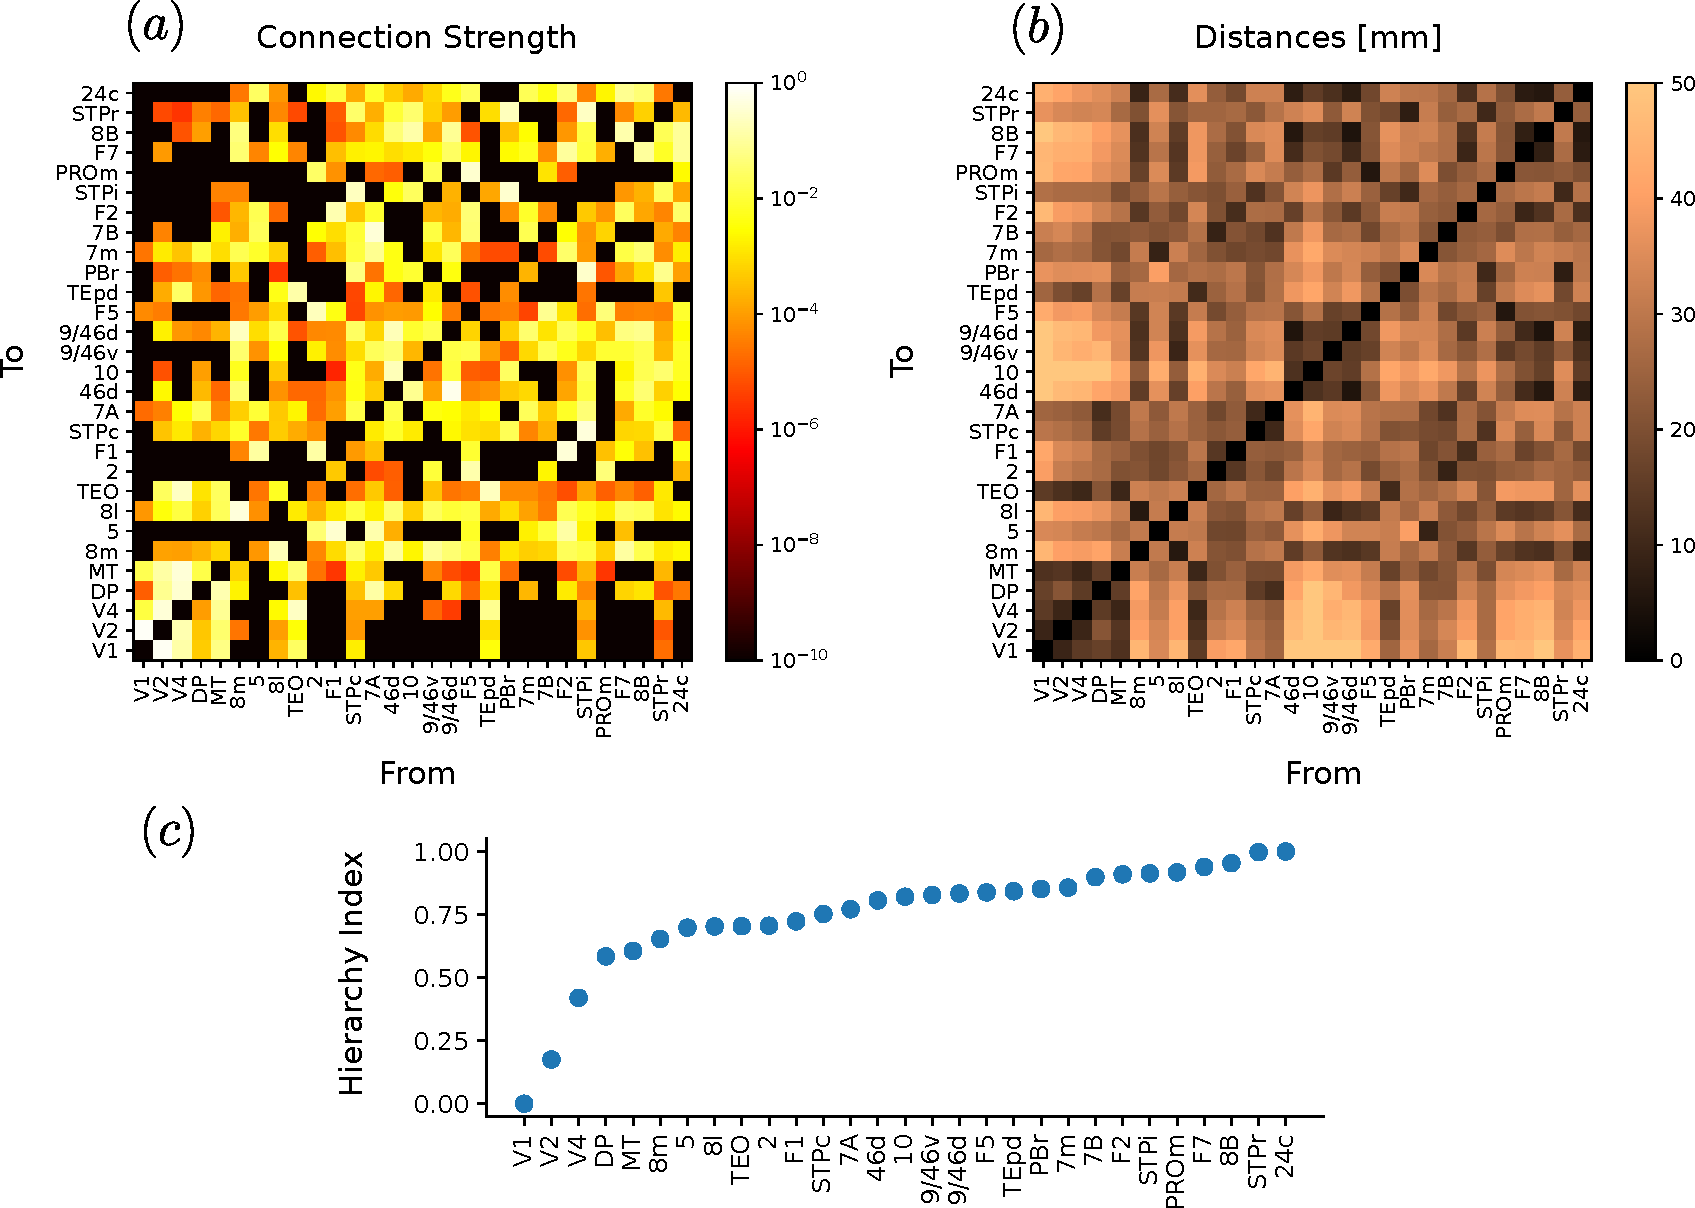
\includegraphics[scale=0.5]{figures/fig_markov.pdf}
 \caption{Data from Markov et. al., \cite{markov2014b} used to build the large-scale networks. In (a) we show the FLN in logarithmic scale due to the large range of values encountered (non-existent connections are shown in black), in (b) the wring distance between cortical areas, and in (c) the normalized anatomical hierarchy of each cortical area.}\label{fig:fig_data}
\end{figure}

Henceforth, we will denote a pair of cortical areas by the indexes $i$, and $j$, in such a way that FLN$_{ij}$ is the FLN from area $i$ to area $j$. Note that, since the graph given by the weighted matrix in Fig.~\ref{fig:fig_data}(a) is asymmetric, FLN$_{ij} \ne $ FLN$_{ji}$. The delay will be represent by the letter $D$, and $D_{ij} = D_{ji}$ is the delay between area $i$ and $j$. Similarly, the anatomical hierarchy of area $i$ is denoted by $h_{i}$.


The data used to build the network is available with the code related to this article in: XXXXXX (the original data can be obtained from
\href{core-nets.org/}{http://core-nets.org/}, however it is necessary to properly organize it in order to be able to run the model; in our repository, all the necessary preprocessing is done).

\subsection{Rate based models}\label{rate_model}

Here we describe the rate based model. We reproduce two sets of results from the original paper in which this model is used: namely, Fig.~$1$, and Fig.~$3$ from \cite{joglekar2018inter}.

\subsubsection{Population dynamics}\label{rate_pop}

The population dynamics of the rate based model is given by Eq.~\ref{eq:rate_general}

\begin{equation}
    \tau_{E,I}\frac{dr_{E,I}(t)}{dt} = -r_{E,I}(t) + \beta_{E,I}\phi[I_{\rm ext}(t)],
    \label{eq:rate_general}
\end{equation}

\noindent where $r(t)$ is the firing rate of each specific population, the sub-index $E,I$ indicates whether the population is excitatory or inhibitory, $\tau$ is the time constant, $\beta$ is the slope of the frequency-current curve, $I_{\rm ext}$ is the net external input which is the sum of synaptic ($I_{\rm syn}$), injected ($I_{\rm inj}$), and any other input current, and $\phi[x] = \text{max}(x,0)$ is a threshold-linear transfer function.

\subsubsection{Local circuit}\label{local_rate}

The local circuit is composed of an excitatory and an inhibitory populations, coupled by an excitatory to inhibitory connection ($E\rightarrow I$), and an inhibitory to excitatory connection ($I\rightarrow E$). In addition, each population is connected to itself, via an $E\rightarrow E$ and an $I\rightarrow I$ couplings. The local circuit described is schematized in Fig.~\ref{fig:fig1}(a), and can be written as:

\begin{equation}
    \begin{split}
            \tau_{E}\frac{dr_{E}(t)}{dt} &= -r_{E}(t) + \beta_{E}\phi[\omega_{EE}r_{E}(t) - \omega_{IE}r_{I}(t) + I_{\rm inj, E}(t)],\\
            \tau_{I}\frac{dr_{I}(t)}{dt} &= -r_{I}(t) + \beta_{I}\phi[\omega_{EI}r_{E}(t) - \omega_{II}r_{I}(t) + I_{\rm inj, I}(t)],
    \end{split}
    \label{eq:rate_local}
\end{equation}

\noindent where $\omega_{ij}$ is the local synaptic weight from $i$ to $j$. $I_{\rm inj, E}$, and $I_{\rm inj, I}$ are external currents injected in the excitatory, and inhibitory populations, respectively.

\subsubsection{Large-scale circuit}\label{lr_rate} The local dynamics of regions within the large-scale network model follows Eq.~\ref{eq:rate_local}. However, regions are now heterogeneous and each of them sees its local weights modulated according to the hierarchical rank of each area. Specifically, the components of the local synaptic currents in area $i$, are given by the following equations:

\begin{equation}
        I^{\rm local,i}_{EE} = \omega_{EE}(1+\eta h_{i})r_E^{i},
        \label{eq:local_ee}
\end{equation}

\begin{equation}
        I^{\rm local,i}_{IE} = -\omega_{IE}r_I^{i}
        \label{eq:local_ie},
\end{equation}

\begin{equation}
        I^{\rm local,i}_{EI} = \omega_{EI}(1+\eta h_{i})r_E^{i}
        \label{eq:local_ei}
\end{equation}

\begin{equation}
        I^{\rm local,i}_{II} = -\omega_{II}r_I^{i},
        \label{eq:local_ii}
\end{equation}

\noindent Intra-regional excitatory currents are  increased by a hierarchy dependent gain factor, in which a parameter $\eta$ multiplies the hierarchical rank index of the considered areas. Consequently, regions with a higher hierarchical order are more excitable.

The long-range synaptic projections are considered to be purely excitatory and their strength are determined by the weighted graph presented in Section~\ref{netowork}. In practice, if the FLN between area $i$ and $j$ is greater than zero (FLN$_{ij} > 0$), those areas are connected. The total long-range synaptic currents that the excitatory and inhibitory populations of area $i$ receive are given by Eqs.~\ref{eq:lr_ee}-\ref{eq:lr_ei}.

\begin{equation}
    I^{lr,i}_{EE} = \mu_{EE}(1+\eta h_{i})\sum_{\substack{j = 0\\i \ne j}}^{N_{\rm areas}}\text{FLN}_{ji}r_{E}^{j},
    \label{eq:lr_ee}
\end{equation}

\begin{equation}
    I^{lr,i}_{EI} = \mu_{EI}(1+\eta h_{i})\sum_{\substack{j = 0\\i \ne j}}^{N_{\rm areas}}\text{FLN}_{ji}r_{E}^{j},
    \label{eq:lr_ei}
\end{equation}

\noindent where $\mu$  represents the long-range synaptic weights, and $N_{\rm areas}$ is the number of cortical areas. Note that the long-range connections are scaled by the hierarchical position of the target regions.

The total current received by the excitatory and inhibitory populations in an area $i$ can be expressed by combining Eqs.~\ref{eq:local_ee}-\ref{eq:lr_ei}, as follows:

\begin{equation}
    I^{i}_{E} = I_{EE}^{local,i} + I^{lr,i}_{EE} + I^{\rm local,i}_{IE} + I_{\rm inj, E}^{i},
    \label{eq:total_current_e}
\end{equation}

\begin{equation}
    I^{i}_{I} = I_{EI}^{local,i} + I^{lr,i}_{EI} + I^{\rm local,i}_{II} + I_{\rm inj, I}^{i},
    \label{eq:total_current_i}
\end{equation}

The transmission delay ($D_{ij}$) between areas $i$ and $j$ is neglected and considered to be instantaneous ($D_{ij}=0$, $\forall$  $i$ and $j$), so that no use is made of the tract length matrix of Fig.~\ref{fig:fig_data}b, but only of the FLN matrix of Fig.~\ref{fig:fig_data}a and the hierarchical order of Fig.~\ref{fig:fig_data}c. 


\subsection{Spiking neuron models}\label{spike_model}

In this section, we describe the spiking neuron network models. Based on them, we reproduced the results of Fig.~$5$, and Fig.~$6$ from the original paper.

\subsubsection{Single neuron}\label{lif_single} Neurons were modeled using the leaky integrate-and-fire (LIF) model  as
follows.

\begin{equation}
\frac{dV(t)}{dt} = -\frac{V(t) - V_{\rm r}}{\tau_{E,I}} + \frac{I_{\rm ext}(t)}{C_{E,I}},
\label{eq:lif_din}
\end{equation}  

\noindent where $V(t)$ is the time-dependent membrane potential, $V_r$ is the resting potential, $\tau$ is the membrane time constant, and $C$ is the membrane capacitance. The external current is given by $I_{\rm ext} = I_{\rm syn} + I_{\rm inj}$, where $I_{\rm syn}$ is the synaptic, and  $I_{\rm inj}$ the injected currents.

A spike is emitted following the spike-and-reset rule in Eq.~\ref{eq::lif_reset}:

\begin{equation}
V(t) \geq V_{\text{th}} \Rightarrow
\begin{cases}
\textrm{Spike at time $t$}\\
V(t + \tau_{\text{ref}}) = V_{\text{reset}},
\end{cases}
\label{eq::lif_reset}
\end{equation}

\noindent  where $V_{\rm th}$ is the spike threshold, $\tau_{\rm ref}$ is the refractory period, and $V_{\rm reset}$ is the reset value of the membrane potential. In Table~\ref{tab:table_lif}, we show the parameters used for the LIF neuron.

\begin{table}[!ht]
\centering
\begin{tabular}{|c|c|c|c|c|c|c|c|}
\hline
$V_{\rm r}$ {[}mV{]} & $V_{\rm reset}$ {[}mV{]} & $V(0)$ {[}mV{]} & $\tau_{E}$ {[}ms{]} & $\tau_{I}$ {[}ms{]} & $\tau_{\rm ref}$ {[}ms{]} & $C_{E}$ {[}pA{]} & $C_{I}$ {[}pA{]} \\ \hline
-70.0                & -60.0                    & -70.0           & 20.0                & 10.0                & 2.0                       & 400.0            & 200.0            \\ \hline
\end{tabular}
\caption{Parameters for the LIF neuron model in Eqs.~\ref{eq:lif_din}-\ref{eq::lif_reset}.}\label{tab:table_lif}
\end{table}



\subsubsection{Local circuit}\label{local_circuit_spk} The local circuit in each spiking region is composed of $N=N_E+N_I=2000$ LIF neurons, where $N_E = 1600$ are excitatory, and $N_I = 400$ are inhibitory. Connections are random and sparse, established with a fixed probability for each pair of neurons set as $p=0.1$. The synaptic current received by the neuron $i$ is given by:

\begin{equation}
I_{\rm syn}^{i} =  \sum_{j} \omega_{ji}\sum_{k}\delta(t-t_{j}^{k}-d),
\label{eqn:syn_delta}
\end{equation}

\noindent  where $\omega_{ji}$ is the synaptic weight from neuron $j$ to neuron $i$, $t_{j}^{k}$ is the time of the $k^{\rm th}$ spike from neuron $j$, and $d$ is the local delay. The input spike-trains are mathematically represented as the sum of Dirac delta terms. 

The local synaptic currents are obtained by replacing the rates $r_E$, and $r_I$ in Eqs.~\ref{eq:local_ee}-\ref{eq:local_ii} with the input spike trains from Eq.~\ref{eqn:syn_delta}. The total local synaptic current received by an excitatory neuron in area $i$ is obtained by combining Eqs.~\ref{eq:local_ee_spk}-\ref{eq:local_ie_spk}:


\begin{equation}
        I^{\rm local,i}_{EE} = \sum_{j=0}^{N_{E}^{\rm pre}}\omega_{EE}(1+\eta h_{i})\sum_{k}\delta(t-t_{j}^{k}-d),
     \label{eq:local_ee_spk}
\end{equation}

\begin{equation}
        I^{\rm local,i}_{IE} = -\sum_{j=0}^{N_{I}^{\rm pre}}\omega_{IE}\sum_{k}\delta(t-t_{j}^{k}-d),
        \label{eq:local_ie_spk},
\end{equation}

\noindent and the total local synaptic current received by an inhibitory neuron in area $i$ is given by Eqs.~\ref{eq:local_ei_spk}-\ref{eq:local_ii_spk}.

\begin{equation}
        I^{\rm local,i}_{EI} = \sum_{j=0}^{N_{E}^{\rm pre}}\omega_{EI}(1+\eta h_{i})\sum_{k}\delta(t-t_{j}^{k}-d),
        \label{eq:local_ei_spk}
\end{equation}

\begin{equation}
        I^{\rm local,i}_{II} = -\sum_{j=0}^{N_{I}^{\rm pre}}\omega_{II}\sum_{k}\delta(t-t_{j}^{k}-d),
        \label{eq:local_ii_spk}
\end{equation}

\noindent In the expression above, $N_E^{\rm pre}$, and $N_I^{\rm pre}$ are the number of excitatory and inhibitory pre-synaptic neurons, respectively.

\subsubsection{Large-scale circuit}\label{lr_spk} Each region is modeled as the local circuit described above. Their long-range synaptic currents received by excitatory and inhibitory neurons in area $i$ from neurons in area $j$, are given by:

\begin{equation}
    I^{lr,i}_{EE} = \sum_{j=0}^{N_E^{\rm pre}}\mu_{EE}(1+\eta h_{i})\text{FLN}_{ji}\sum_{k}\delta(t-t_{j}^{k}-D^{'}_{ji}),
    \label{eq:lr_ee_spk}
\end{equation}

\begin{equation}
    I^{lr,i}_{EI} = \sum_{j=0}^{N_E^{\rm pre}}\mu_{EI}(1+\eta h_{i})\text{FLN}_{ji}\sum_{k}\delta(t-t_{j}^{k}-D^{'}_{ji}),
    \label{eq:lr_ei_spk}
\end{equation}

\noindent  The delays $D^{'}_{ji}$ are sampled from normal distribution with mean $D_{ji}$, and standard deviation $0.1D_{ij}$ ($D^{'}_{ji} = \mathcal{N}(D_{ji}, 0.1D_{ji})$). These delays were estimated dividing the tract lengths (Fig.~\ref{fig:fig1}b) by the propagation velocity of $v=3.5$ m/s. 

The hierarchical order of the targeted region is scaled via a gain parameter $\eta$. All the parameters used in the model of a large-scale circuit described above are given in Table~\ref{tab:par_spike}.

\subsection{Balanced amplification}\label{gba}

As we briefly mentioned in Section~\ref{introduction}, the models described above were used to study signal propagation in the cortical system. In Joglekar et. al., \cite{joglekar2018inter}, the mechanism of \emph{balanced amplification}, is hypothesised to contribute to reliable signal propagation through the cortical hierarchy.

For the local circuits, and \ref{local_circuit_spk}) this mechanism is refereed to as \emph{local} balanced amplification (LBA), and consists of increasing the recurrent excitation ($\omega_{EE}$), and the lateral inhibition ($\omega_{IE}$). For the large-scale circuits this mechanism is referred to as \emph{global} balanced amplification (GBA), and consists of increasing the long-range $E\rightarrow E$ excitation  ($\mu_{EE}$), and the local lateral inhibition ($\omega_{IE}$).

These balanced amplification mechanisms, when activated, can achieve two effects: first, through the increase of excitatory couplings, signal transmission among areas is enhanced; and, second, increasing the lateral inhibition within local circuits, network instability is avoided, despite the overall increase in excitation.

In the results we will compare signal propagation in the models above in two alternative regimes, corresponding to two distinct functional states of the brain network: (i) Weak LBA/GBA, and (ii) Strong LBA/GBA. The transition from regime (i) to (ii) is done via increasing $\omega_{EE}/\mu_{EE}$, and $\omega_{IE}$, as described above. The parameters used in each regime are specified in the specifically associated results section.


\section{Results}

In this Section we will present the results we choose to replicate from the original article. These results give an outlook of the  mechanism of global balanced amplification (Section~\ref{gba}). In Sections~\ref{lba_result}-\ref{gba_spk}
 we replicate the result in Figures~$1$, $3$, $5$ and $6$ from Joglekar et. al. \cite{joglekar2018inter}.  For each result we also highlight the issues we had replicating it, such as the parameters values not informed in the original publication. The name of those parameters  will be coloured red in the parameter Tables~\ref{tab:tab1}-\ref{tab:par_spike}.

\subsection{Local Balanced Amplification in an Inhibition-Stabilized Local Circuit}\label{lba_result}

To reproduce a first result in Figure 1 of the original \cite{joglekar2018inter} paper, we use the local circuit described by the rate based model of Eq.~\ref{eq:rate_local}. In Fig.~\ref{fig:fig1}(a), we show a schematic representation of this simple circuit. The parameters for the used model are given in Table~\ref{tab:tab1} of this article. All parameters were copied from the original publication, apart from $\tau_{E}$ and $\tau_{I}$ for which we could not find an explicit value in the original publication. However, in line with descriptions and Equation~1 therein, we set  $\tau_{E} = \tau_{I}= \tau$ and adjusted this common value $\tau$ to get figures looking similar to the original ones. The estimated value is the one we report in Table~\ref{tab:tab1}, together with the other parameters.

This first result we reproduce exemplify the mechanism of  balanced amplification within a local circuit. In Fig.~\ref{fig:fig1}(b), we show the evolution of the excitatory rate $r_E(t)$, starting from the initial condition $r_E(0) = 1$, and $r_I(0) = 0$. This initial condition emulates the state in which the E population is already active due to a transient input. The green and violet curves correspond to the E rate evolution in a weak and strong LBA conditions. Note that the response of the system is indeed enhanced in the strong LBA case, leading to evoked activity which has both a stronger peak amplitude and an enhanced transient.


\begin{figure}[!ht]
 \centering
 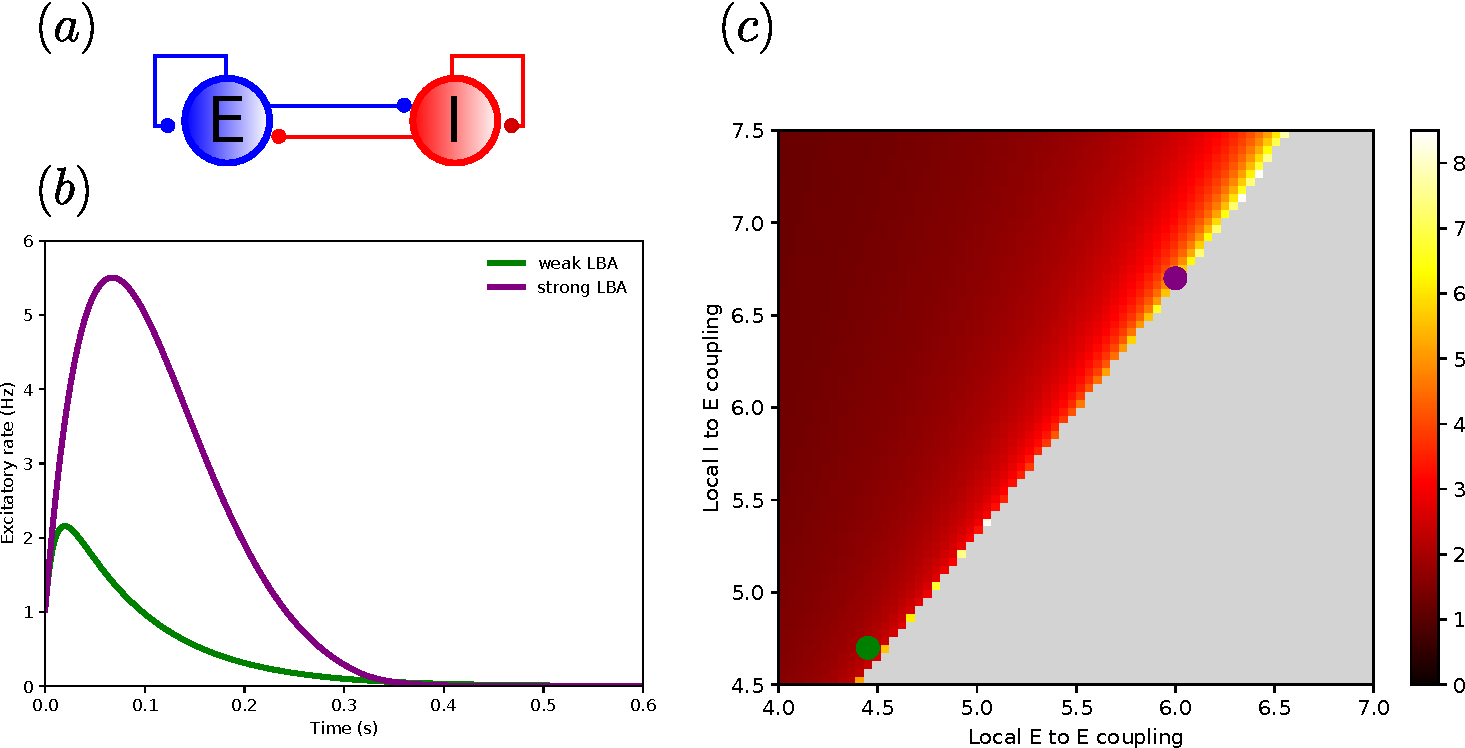
\includegraphics[scale=0.4]{figures/fig1.pdf}
 \caption{Replication of the result in Figure~1 of the original publication \cite{joglekar2018inter}. In (a) we show a schematic depiction of the local circuit used to generate the results, in (b) we show the response rate of the excitatory population after its initial value being set to $1$ Hz (emulating application of a brief destabilizing input), for weak (green) and strong (purple) local balanced amplification (LBA). In (c), we show the peak rate of the excitatory population as a function of $\omega_{EE}$, and $\omega_{IE}$, where the green and purple circles indicate the points used to produce the curves in (b) (corresponding, respectively, to the used weak and strong LBA conditions) }\label{fig:fig1}
\end{figure}

To illustrate the mechanism of LBA, in Fig.\ref{fig:fig1}(c) we show the peak response of the excitatory population as a function of the internal couplings $\omega_{EE}$, and $\omega_{IE}$. The regions where the excitatory rate diverge are shown in gray. As it can be seen, a high increase of $\omega_{EE}$ destabilizes the circuit making its rate explode, however as $\omega_{IE}$ increases, larger values of  $\omega_{EE}$ can be tolerated before triggering a rate instability. Remark that both the weak and strong LBA working points lie at the slightly sub-critical edge of this rate instability. We consider that the replication of this result was successful, despite one of the parameters in Table~\ref{tab:tab1} had to be estimated.

\begin{table}[!ht]
\centering
\begin{tabular}{|c|c|c|}

\hline
                    & \textbf{Weak LBA} & \textbf{Strong LBA} \\ \hline
$\omega_{EI}$ [pA/Hz] & \multicolumn{2}{c|}{4.29}               \\ \hline
$\omega_{II}$ [pA/Hz] & \multicolumn{2}{c|}{4.71}               \\ \hline
$\beta_{E}$         & \multicolumn{2}{c|}{1.00}               \\ \hline
$\beta_{I}$         & \multicolumn{2}{c|}{1.00}               \\ \hline
$r_E(0)$ [Hz]           & \multicolumn{2}{c|}{1.00}               \\ \hline
$r_I(0)$ [Hz]           & \multicolumn{2}{c|}{0.00}               \\ \hline
\textcolor{red}{$\tau$ [ms]}           & 20.0              & 30.0                \\ \hline
$\omega_{EE}$ [pA/Hz] & 4.45              & 6.00                \\ \hline
$\omega_{IE}$ [pA/Hz] & 4.70              & 6.70                \\ \hline
\end{tabular}
\caption{Parameters used in Eq.~\ref{eq:rate_local} to produce the results in Fig.~\ref{fig:fig1}. For the parameters in red we could not find a value in the original publication and we had therefore to guess values allowing the reproduction of the published results. Note that we have used $\tau_{E} = \tau_{I} = \tau$.}\label{tab:tab1}
\end{table}

\subsection{Global Balanced Amplification
in the Large-Scale Model Improves Signal Propagation}\label{gba_rate}

Next, we study the propagation of an input pulse in the network composed of $29$ cortical areas \cite{markov2014b} (Section~\ref{netowork}), where each node comprises an E and I population of rate based model (Section~\ref{rate_model}). All the parameters used for the model are given in Table~\ref{tab:tab2}.

In Fig.~\ref{fig:fig2}(a,b) we show a schematic representation of the connection between two cortical areas, for the weak and strong GBA cases. The increase in $\mu_{EE}$ and $\omega_{IE}$ for the strong GBA conditions is represented by the thickness of the arrows for these connections in  Fig.~\ref{fig:fig2}(b).

\begin{figure}[!hb]
 \centering
 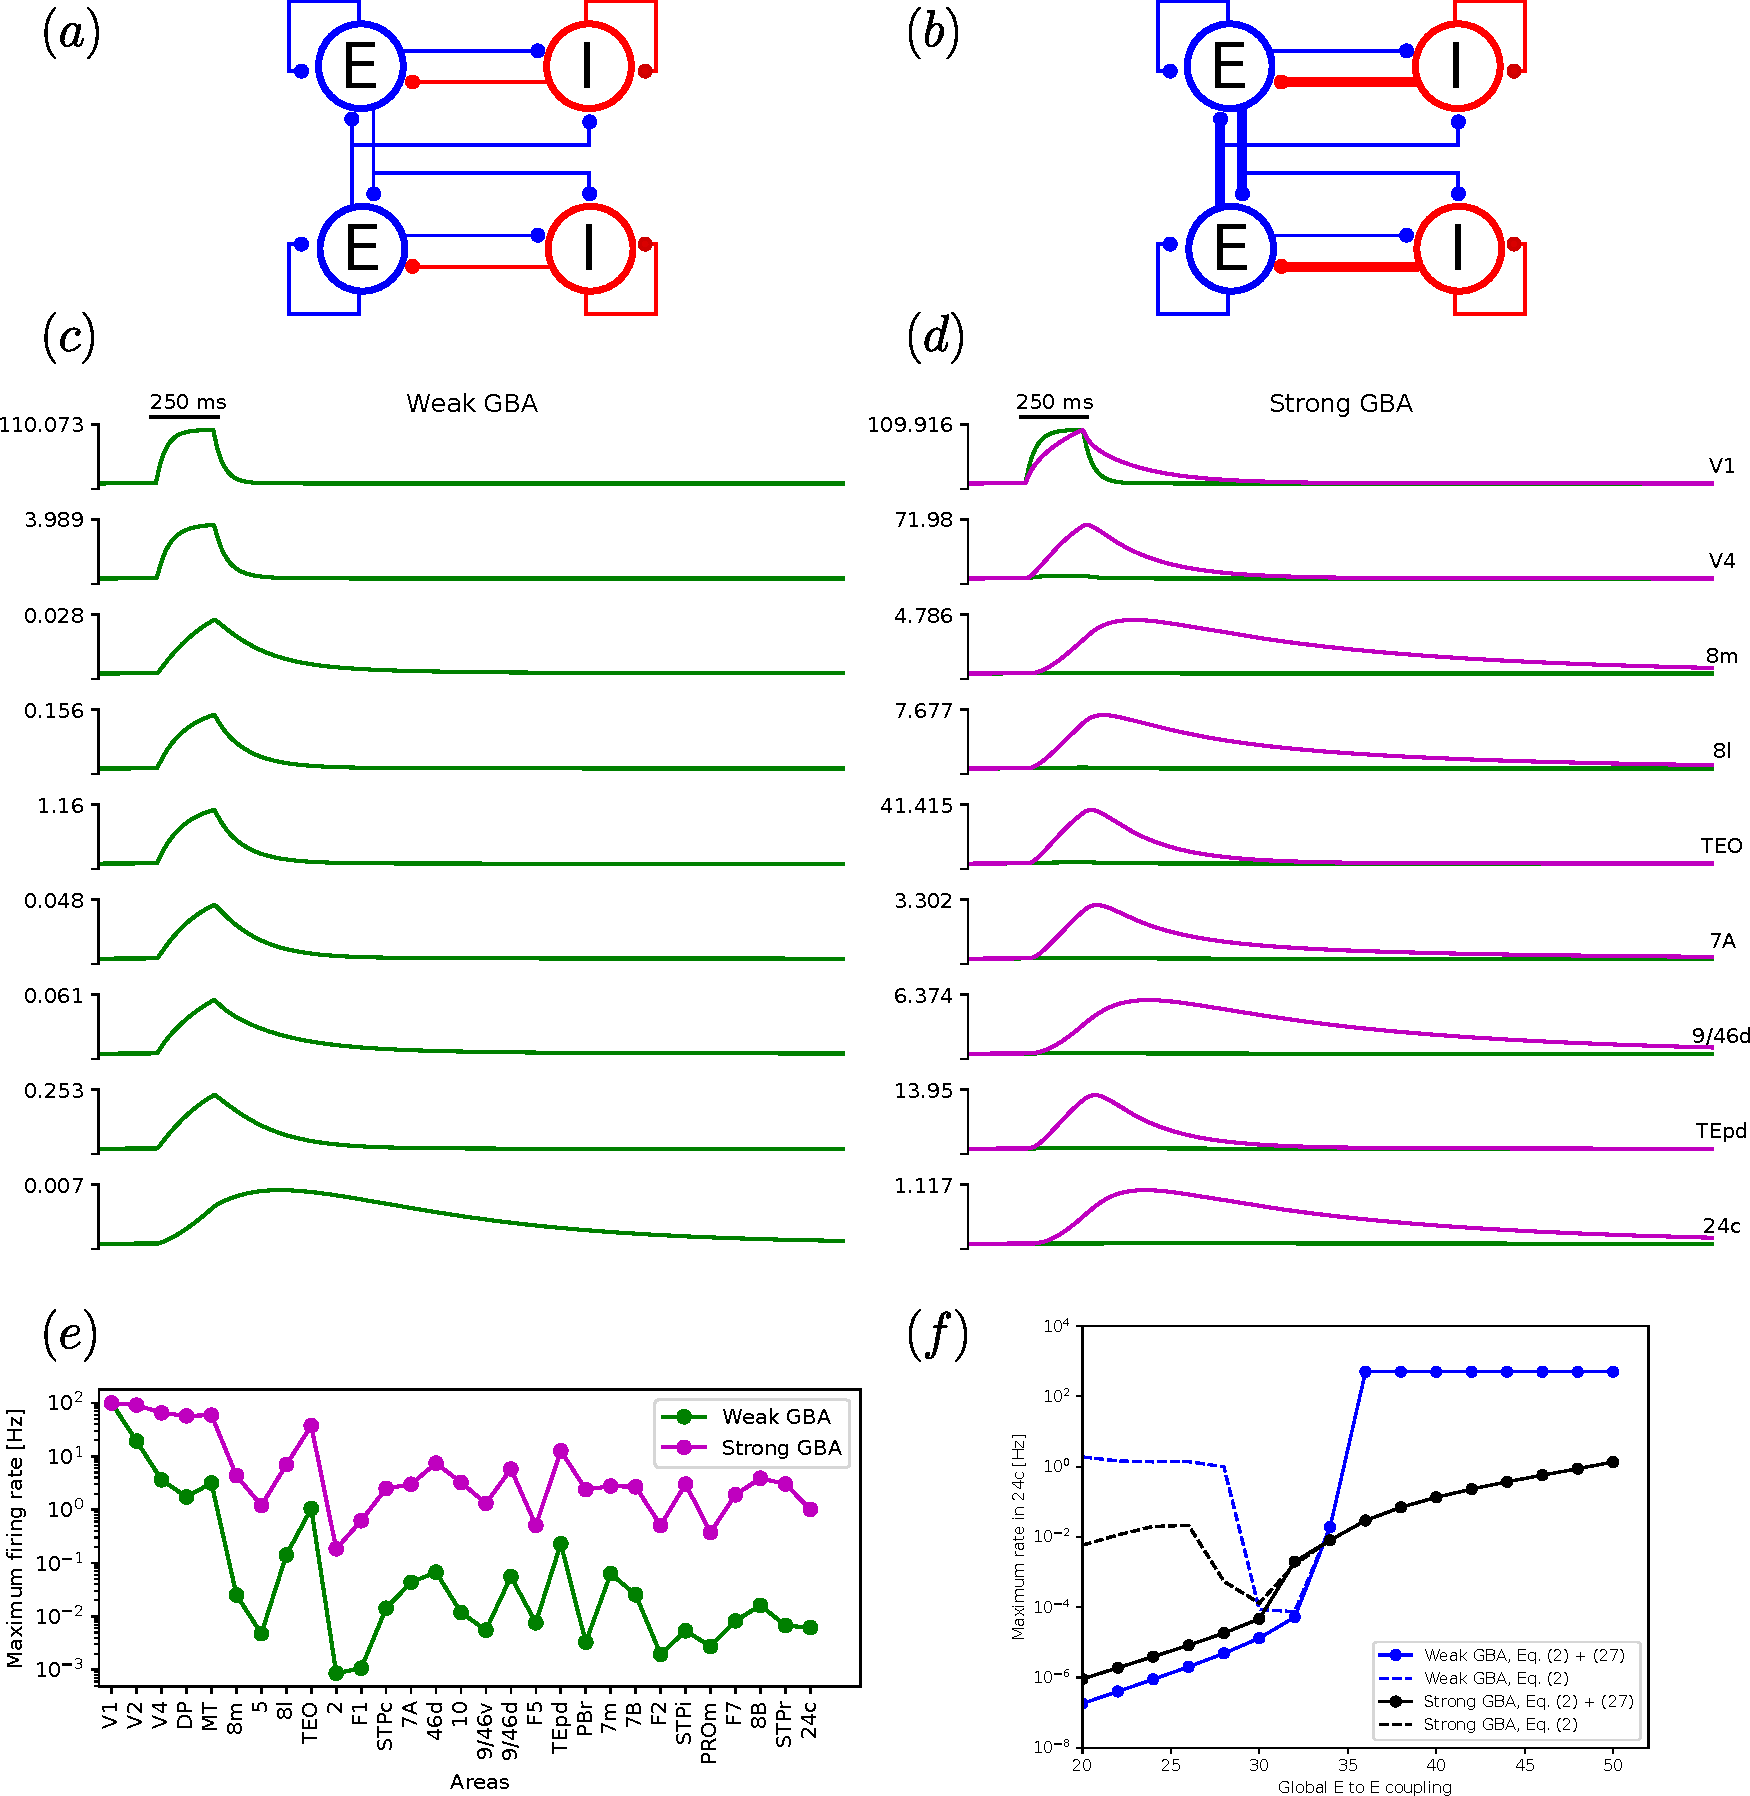
\includegraphics[scale=0.4]{figures/fig3.pdf}
 \caption{Reproduction of Figure 3 from the original paper \cite{joglekar2018inter}. In (a) and (b), we show inter-regional coupling within the large-scale connectome model for the regimes of weak and strong Global Balanced Amplification (GBA). In (c) and (d), we show propagating pulses of response to a stimulus injected in region V1, in regions with increasing hierarchy. Responses in (d) are sustained for longer times in certain regions and stronger in amplitude (the green lines in (d) correspond to the lines in (c), remark the changed vertical time-scale). The increase in peak response in strong vs weak GBA is also visualized for all regions in (e), in (f) we show the maximum excitatory rate at area 24c for weak (blue) and strong (black) GBA, the solid lines correspond to the simulations using the correction given by Eq.~\ref{eq:migue}.}\label{fig:fig2}
\end{figure}

For each area $i$ a background input is inject to the excitatory ($I_{BG,E}^{i}$) and inhibitory ($I_{BG,I}^{i}$)  populations in order to maintain a background rate of $r_E^{\rm BG} = 10$ Hz in the first and $r_I^{\rm BG} = 35$ Hz in the latter. The initial firing rates are set as being equal to the background rate.

To compute $I_{BG,E}^{i}$ and $I_{BG,I}^{i}$, first let $\pmb W_{EE}$, $\pmb W_{IE}$, $\pmb W_{EI}$ and $\pmb W_{II}$ be square matrices with size $N_{\rm areas}$. Then, using $M^{ij}$ to denote the element in row $i$ and column $j$ from a given matrix $M$, we can compute each element from those matrices as:

\begin{equation}
W_{EE}^{ij} \Rightarrow
\begin{cases}
\mu_{EE}(1+\eta h_{i})\text{FLN}_{ji}, \text{ if } i \neq j,\\
-1 + \omega_{EE}(1+\eta h_{i}), \text{ if } i = j,
\end{cases}
\label{eq::wee}
\end{equation}

\begin{equation}
W_{IE}^{ij} \Rightarrow
\begin{cases}
0, \text{ if } i \neq j,\\
-\omega_{IE}, \text{ if } i = j,
\end{cases}
\label{eq::wie}
\end{equation}

\begin{equation}
W_{EI}^{ij} \Rightarrow
\begin{cases}
\mu_{EI}(1+\eta h_{i})\text{FLN}_{ji}, \text{ if } i \neq j,\\
\omega_{EI}(1+\eta h_{i}), \text{ if } i = j,
\end{cases}
\label{eq::wei}
\end{equation}

\noindent and,

\begin{equation}
W_{II}^{ij} \Rightarrow
\begin{cases}
0, \text{ if } i \neq j,\\
-1 + \omega_{II}, \text{ if } i = j.
\end{cases}
\label{eq::wii}
\end{equation}

Next we define the square matrix $\pmb A$ with size $2N_{\rm areas}$:


\begin{equation}
    \pmb A = \begin{bmatrix} 
                    \pmb W_{EE} & \pmb W_{IE} \\
                    \pmb W_{EI}& \pmb W_{II}
                 \end{bmatrix} ,
\end{equation}

\noindent and $\pmb B$ a matrix with dimensions $[2N_{\rm areas}, 1]$, where $B^{i} = r_{E}^{\rm BG}$ for $i < N_{\rm areas}$, otherwise $B^{i} = r_{I}^{\rm BG}$. The background currents are computed as:

\begin{equation}
    \pmb I_{BG} = -\pmb A \times \pmb B,
\end{equation}

\noindent where $\times$ is the matrix multiplication, $I_{BG,E}^{i}$, and $I_{BG,I}^{i}$ are given by:

\begin{equation}
\begin{cases}
I_{BG,E}^{i}  = I_{BG}^{i}, \text{ if } i < N_{\rm areas},\\
I_{BG,I}^{i-N_{\rm areas}}  = I_{BG}^{i}, \text{ if } i \geq N_{\rm areas}.
\end{cases}
\label{eq::ibge}
\end{equation}

Such procedure lead to determine parameters associated to the steady-state working point of the network. For exact derivation, of Eq.~\ref{eq::ibge} see \cite{joglekar2018inter} star methods section.


To simulate the signal propagation, an input is injected in the excitatory population of the primary visual cortex (V1) for $t_{\rm durr} = 225$ ms, from $t_{i} = 200$ ms to $t_{f} = 225$ ms. For the weak GBA the input injected in V1 was $I_{\rm inj, E}^{\rm V1} = 41.90$ pA/Hz and for the strong GBA  $I_{\rm inj, E}^{\rm V1} = 21.93$ pA/Hz.

The input injected to area V1 is attenuated of factor larger than $10,000$ times as it reaches area 24c in the weak GBA, while for the strong GBA the attenuation is approximately of only $100$ times (Fig.~\ref{fig:fig2}(c,d)). The enhancement in signal propagation can also be tracked by looking at the peak firing rate in each cortical area after the input was injected in V1. In Fig.~\ref{fig:fig2}(e), we show the peak response rate in each region for both the weak and strong GBA regimes. The plot is in logarithmic scale manifesting the large level of boosted propagation to higher hierarchical order areas.

Finally, in Fig.~\ref{fig:fig2}(f), we measured the maximum response firing rate in area 24c (highest hierarchical order) as a function of the long-range coupling scale $\mu_{EE}$, the the weak and strong GBA cases. For both conditions, we use the same parameters as for the weak GBA in Fig.~\ref{fig:fig2}(c), and the values of $\mu_{EE}$ used go from $20$ pA/Hz to $50$ pA/Hz with a step of $2$ pA/Hz. For the strong GBA we have increased $\omega_{IE}$ using the following rule: $\omega_{IE} = 19.7 + 0.31\mu_{EE}$, that was set manually based on the ranges used in their Matlab source code (see bellow).

The first result we obtained is shown by the dashed lines in Fig.~\ref{fig:fig2}(f). For values of $\mu_{EE} < 30$ pA/Hz, the obtained result diverged from the original one and we obtained greater peak firing rates in area 24c.

We were able to retrieve the original results, shown in solid lines in Fig.~\ref{fig:fig2}(f), by introducing the following condition while solving the rate equations numerically:

\begin{equation}
    \text{If } r_{E,I}(t) < r_{E,I}^{\rm BG}, \text{ then } r_{E,I}(t) = r_{E,I}^{\rm BG}.
    \label{eq:migue}
\end{equation}

This condition was not mentioned in the original article. However it was found in the Matlab implementation of the model, publicly available  at the GitHub repository : \href{github.com/xjwanglab/JoglekarEtAl2018_Neuron}{github.com/xjwanglab/JoglekarEtAl2018\_Neuron} (unreferenced in \cite{joglekar2018inter}).

Such adjustment guarantees that the firing rates of any population in the model do not go below their baseline activity, causing some of the populations to be effectively ``switched off''. In absence of this condition, some of the inhibitory populations would become too silent, reducing the overall level of inhibition and thus causing some rates to increase in an unbalanced way (hence the larger peak response rate in area 24c). 

The condition in Eq.~\ref{eq:migue} was not mentioned in the original publication. In order to be able to reproduce this result we made a modification to NEST source code, adding the possibility to set the condition given in Eq.~\ref{eq:migue} as an option for the rate model available in NEST. This resulted in a pull-request that was integrated as the model ``threshold\_lin\_rate'' in NEST from version 3.0 \cite{hahne_jan_2021_4739103}. For this reason it is recommended to use this updated version when attempting to run our simulation codes.


\begin{table}[!hp]
\centering
\begin{tabular}{|c|cc|}
\hline
                             & \multicolumn{1}{c|}{\textbf{Weak GBA}} & \textbf{Strong GBA} \\ \hline
$\omega_{EI}$ {[}pA/Hz{]}    & \multicolumn{2}{c|}{12.5}                                    \\ \hline
$\omega_{II}$ {[}pA/Hz{]}    & \multicolumn{2}{c|}{12.5}                                    \\ \hline
$\omega_{EE}$ {[}pA/Hz{]}    & \multicolumn{2}{c|}{24.3}                                    \\ \hline
$\mu_{EI}$ {[}pA/Hz{]}       & \multicolumn{2}{c|}{25.3}                                    \\ \hline
$\beta_E/\beta_I$            & \multicolumn{2}{c|}{0.066/0.351}                             \\ \hline
$r_E^{BG}/r_I^{BG}$ {[}Hz{]} & \multicolumn{2}{c|}{10/35}                             \\ \hline
$r_E(0)/r_I(0)$ {[}Hz{]}     & \multicolumn{2}{c|}{10/35}                                   \\ \hline
$\tau_E/\tau_I${[}ms{]}      & \multicolumn{2}{c|}{20/10}                                   \\ \hline
$\eta$                       & \multicolumn{2}{c|}{0.68}                                    \\ \hline
$\tau_i/\tau_f$ {[}ms{]}     & \multicolumn{2}{c|}{200/225}                                 \\ \hline
$\omega_{IE}$ {[}pA/Hz{]}    & \multicolumn{1}{c|}{19.7}              & 25.2                \\ \hline
$\mu_{EE}$ {[}pA/Hz{]}       & \multicolumn{1}{c|}{33.7}              & 51.5                \\ \hline
$I_{inj,E}^{V1}$ {[}pA/Hz{]} & \multicolumn{1}{c|}{41.90}             & 21.93               \\ \hline
\end{tabular}
\caption{Parameters used for the large-scale rate based model described in Section~\ref{lr_rate}, to produce the results in Fig.~\ref{fig:fig2}. }\label{tab:tab2}
\end{table}

%\begin{table}[!hp]
%\centering
%\begin{tabular}{|c|c|c|c|c|}
%\hline
%                               & \textbf{}   &                                 & \textbf{Weak GBA} & \textbf{Strong GBA} \\ \hline
%$\omega_{EI}$ [pA/Hz]            & 12.2        & $\omega_{IE}$ [pA/Hz]             & 19.7              & 25.2                \\ \hline
%$\omega_{II}$ [pA/Hz]            & 12.5        & $\mu_{EE}$ [pA/Hz]                & 33.7              & 51.5                \\ \hline
%$\omega_{EE}$ [pA/Hz]            & 24.3        & $I_{\rm inj, E}^{\rm V1}$ [pA/Hz] & 41.90             & 21.93               \\ \hline
%$\mu_{EI}$ [pA/Hz]               & 25.3        &                                 &                   &                     \\ \hline
%$\beta_{E}/\beta_{I}$          & 0.066/0.351 &                                 &                   &                     \\ \hline
%$r_E^{\rm BG}/r_I^{\rm BG}$ [Hz] & 10/35       &                                 &                   &                     \\ \hline
%$r_E(0)/r_I(0)$ [Hz]             & 10/35       &                                 &                   &                     \\ \hline
%$\tau_{E}/\tau_{I}$ [ms]          & 20.0/10.0   &                                 &                   &                     \\ \hline
%$\eta$                         & 0.68        &                                 &                   &                     \\ \hline
%$t_{i}/t_{f}$ [ms]               & 200/225     &                                 &                   &                     \\ \hline
%\end{tabular}
%\caption{Parameters used for the large-scale rate based model described in Section~\ref{lr_rate}, to produce the results in Fig.~\ref{fig:fig2}. }\label{tab:tab2}
%\end{table}

Overall, we were able to replicate the behavior of the reference model. However, concerning the specific result of Fig.~\ref{fig:fig2}(f), the original result could be reproduced only adding the ad hoc but reasonable condition in Eq.~\ref{eq:migue}.


\subsection{Reliable Signal Propagation in a Spiking Network Model}\label{gba_spk}

Next, we continue the analysis of the propagation of an input signal in the large-scale model, but replacing the rate units with the regional spiking network model described in Section~\ref{spike_model}.

We study signal propagation in the spiking large-scale model for two different regimes of the network: (i) asynchronous and (ii) synchronous. In both cases, we perform simulations in both the weak and strong GBA conditions. The parameters for (i) and for (ii) are given in Table~\ref{tab:par_spike}.

The activity of the network is driven by independent white noise background currents injected in all neurons, and given by Eq.~\ref{eq:noise_input}.

\begin{equation}
    I_{BG,E,I}^{i} = \mu_{V,E,I}\frac{C_{E,I}}{\tau_{E,I}} + \sigma_{V} \frac{C_{ E,I}}{\tau_{E,I}}\frac{1+e^{-dt/\tau_{E,I}}}{1-e^{-dt/\tau_{E,I}}}\xi(t),
    \label{eq:noise_input}
\end{equation}

\noindent where $\mu_{V}$ is the average value of the membrane potential, $\sigma_{V}$ is the standard deviation of the noise, both in mV, and $\xi(t)$ is a Gaussian variable with zero mean and unit variance. 

In the original paper, the authors mention that a background input was given to the network in order to maintain the spiking activity of the excitatory population between $0.75-1.5$ Hz and the inhibitory population between $5-6$ Hz. The authors, however, did not explicitly mention the values of $\mu_V$ and $\sigma_{V}$ used (red table entries in Table~\ref{tab:par_spike}). We here tried to reverse-engineer their values via the reproduction of the published results, and we were able to reproduce the specified steady-state rates (Table~\ref{tab:rates}).

\begin{table}[h!]
\centering
\begin{tabular}{|ccc|}
\hline
\multicolumn{3}{|c|}{\textbf{Weak GBA}}                                                                                 \\ \hline
\multicolumn{1}{|c|}{\textbf{Firing rate {[}Hz{]}}} & \multicolumn{1}{c|}{\textbf{Asynchronous}} & \textbf{Synchronous} \\ \hline
\multicolumn{1}{|c|}{\textbf{Excitatory}}           & \multicolumn{1}{c|}{1.30}                  & 0.83                 \\ \hline
\multicolumn{1}{|c|}{\textbf{Inhibitory}}           & \multicolumn{1}{c|}{5.59}                  & 5.62                 \\ \hline
\multicolumn{3}{|c|}{\textbf{Strong GBA}}                                                                               \\ \hline
\multicolumn{1}{|c|}{\textbf{Excitatory}}           & \multicolumn{1}{c|}{1.49}                  & 0.82                 \\ \hline
\multicolumn{1}{|c|}{\textbf{Inhibitory}}           & \multicolumn{1}{c|}{5.99}                  & 5.52                 \\ \hline
\end{tabular}
\caption{Average firing rate for each cell population type and each network state.}\label{tab:rates}
\end{table}

To study signal propagation we injected an external current pulse into all excitatory neurons in V1 ($I_{\rm inj, E}^{\rm V1}$). In the next two sessions we show the results for the asynchronous and synchronous regimes.

\subsubsection{Asynchronous regime}\label{asyncreg}

For the asynchronous regime we injected an input pulse $I_{\rm inj, E}^{\rm V1}$ for $t_{\rm durr} = 150$ ms, from $t_{i} = 500$ ms to $t_{f} = 650$ ms. For the weak GBA $I_{\rm inj, E}^{\rm V1} = 300$ pA, and for the strong GBA $I_{\rm inj, E}^{\rm V1} = 126$ pA.

In Fig.~\ref{fig:fig3}(a,b) we show the raster plot (only excitatory neurons within each area are shown) for the weak and strong GBA conditions. Our result is very similar to the original one. For the weak GBA condition, the signal propagates to a few areas only along the ventral visual stream: V1, V2, V4, TEO and TEpd. In the strong GBA condition, the response to the input injected in V1 is enhanced in those areas, and other areas are reached as well such as: 7A, 46d, 7m and 7B. The arrival time in each area varies due to the used synaptic inter-areal delays in long-range connections.

To show the propagation of the signal to other areas, in Fig.~\ref{fig:fig3}(c) we measure the peak excitatory firing rate between $t_{i}$ and $t_{f}+20$ ms. The maximum firing rates are plot in logarithmic scale and one can observe that they indeed increase for the strong GBA condition, with a near-perfect quantitative matching with the original figure in \cite{joglekar2018inter}. The results about signal propagation in the large-scale spiking network model in the asynchronous regime are  reproduced in our NEST model.

\begin{figure}[!ht]
 \centering
 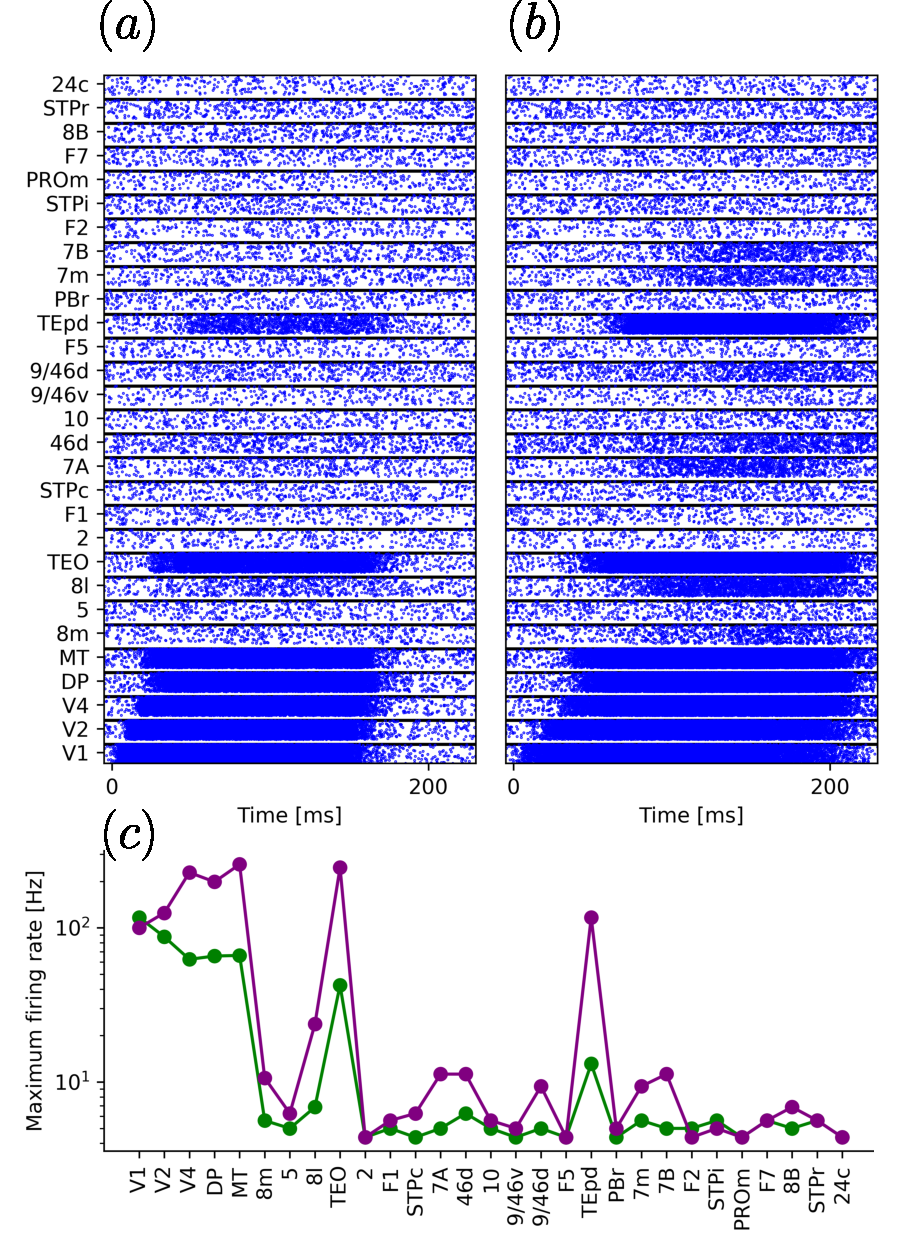
\includegraphics[scale=0.6]{figures/fig5.pdf}
 \caption{Signal propagation in the large-scale spiking neuron network in the asynchronous regime. In (a) we show the network response to a stimulus applied to V1 ($I_{\rm inj, E}^{\rm V1} = 300$ pA) during $150$ ms in the weak GBA. In (b) we show the same but for the strong GBA  condition ($I_{\rm inj, E}^{\rm V1} = 126$ pA). In (c) we show the peak response rate in each region along the cortical hierarchy, after the stimulus injection in V1 for the weak (green), and strong GBA (purple) conditions. }\label{fig:fig3}
\end{figure}


\subsubsection{Synchronous regime}\label{syncreg} For the synchronous regime we injected an input pulse $I_{\rm inj, E}^{\rm V1}$ for $t_{\rm durr} = 8$ ms, from $t_{i} = 500$ ms to $t_{f} = 508$ ms. For the weak GBA $I_{\rm inj, E}^{\rm V1} = 200$ pA and for the strong GBA $I_{\rm inj, E}^{\rm V1} = 200$ pA.

We performed the same analyses as for the asynchronous case. In Fig.~\ref{fig:fig4}(a,b) we show the raster plot for the weak and strong GBA conditions. Qualitatively we got a result very similar to the original one, even though the maximum response rate per regions in Fig.~\ref{fig:fig4}(c) had some quantitative differences. Notably, the response amplification we obtained for hierarchically-intermediate regions as STPc, 7a, 46d and 10 was less strong than in the original model and we did not observe substantial amplification in the highest order regions as STPr and 24c. In general, all rates we obtained in early regions (V1, V2, V4, DP, MT) were stronger than expected.

\begin{figure}[!ht]
 \centering
     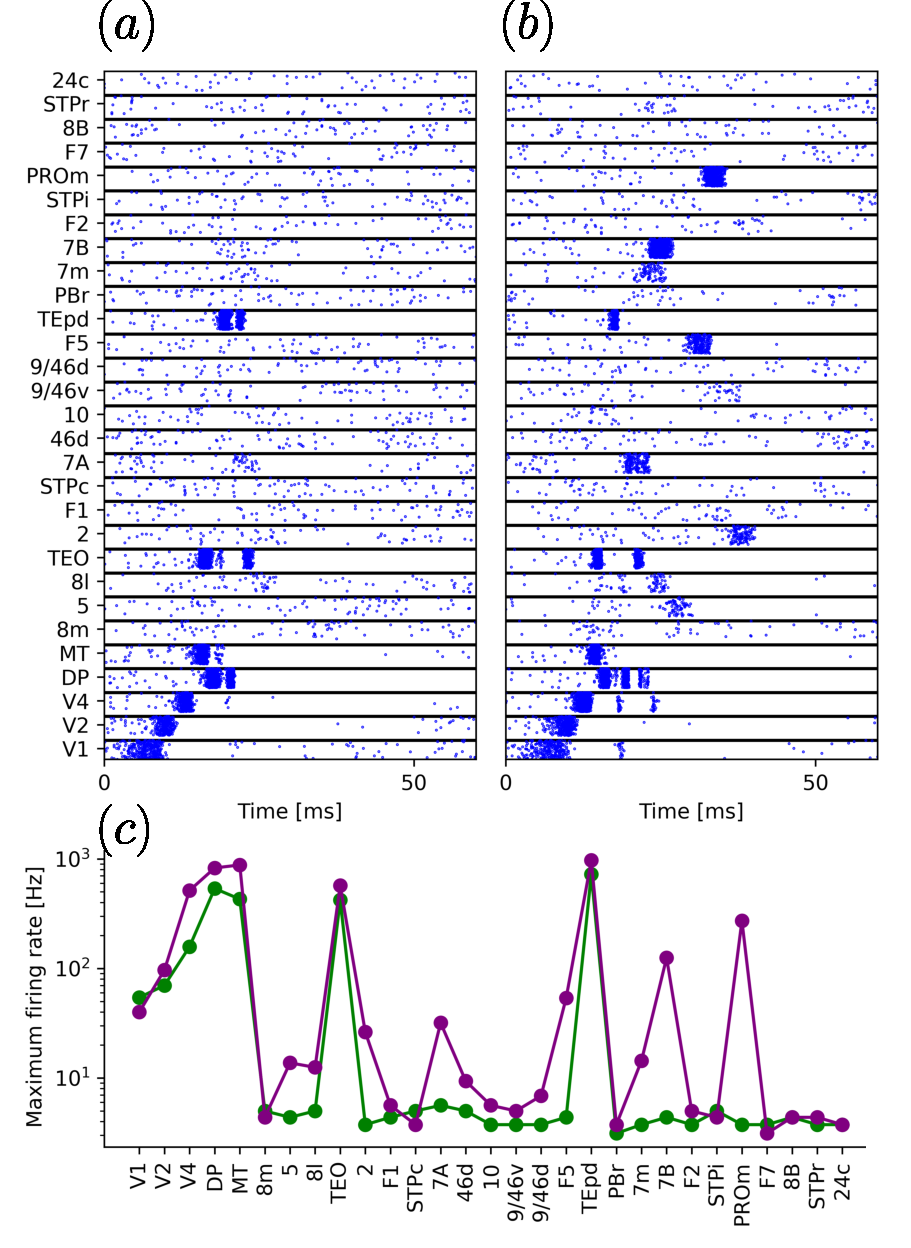
\includegraphics[scale=0.6]{figures/fig6.pdf}
 \caption{Signal propagation in the large-scale spiking neuron network in the synchronous regime. In (a) we show the network's response to a stimulus applied to V1 ($I_{\rm inj, E}^{\rm V1} = 200$ pA) during $8$ ms in the weak GBA condition. In (b) we show the same but for the strong GBA condition  ($I_{\rm inj, E}^{\rm V1} = 200$ pA). In (c), we show the peak frequency in each area after the stimulus injection in V1 for the weak (green), and strong GBA (purple) conditions. }\label{fig:fig4}
\end{figure}

We report in Fig.~\ref{fig:fig4} a simulation with a good semi-quantitative match with the original results. However, we also noticed that the network is highly sensitive to the random seed used to initialize the simulation and this sensibility on initial conditions may explain the quantitative deviations between our response profile and the one shown in the original paper. It is important to note that NEST assigns different seeds to each thread used to simulate the network, therefore, using a different number of threads when running a parallel situation might change the result, making even more difficult to obtain exactly the same raster when repeating the simulation multiple times (for our simulation we have used $20$ threads). Furthermore, we noticed the same phenomenon  when running the original Brian 2 code for this model (data not shown).

Further investigations revealed that the network activity depends on the state set for the random number generator. For Figs.~\ref{fig:fig3}-\ref{fig:fig4}, we run the simulations for a range of random seed values to obtain the expected results. However, changing their values could generate an unstable network. Especially, for the strong GBA and synchronous case, activity can become epileptic-like in some high-order regions, as shown in an example simulation in Fig.~\ref{fig:fig5}. 

\begin{figure}[!ht]
 \centering
     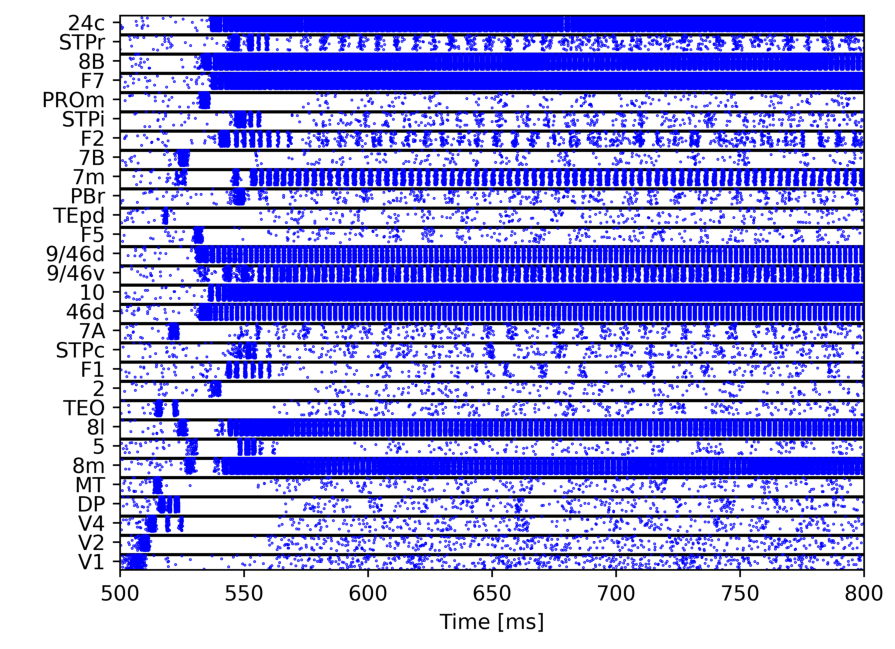
\includegraphics[scale=0.6]{figures/fig7.pdf}
 \caption{Raster plot for the synchronous regime network with strong GBA condition, with all parameters as in Fig.~\ref{fig:fig4}, but with a different choice of random seeds for the parallel simulation. This example raster manifests that, depending on the seed used, the network may become exceedingly unstable.}\label{fig:fig5}
\end{figure}

This suggests, that the synchronous network may be sitting close to a rate instability. Tuning the system to be slightly subcritical is crucial for access to high-hierarchical order regions to take place, as an effect of enhanced GBA. However, we may have been using a too narrow safety margin, or an exceedingly strong input pulse. The simulations we show have been done with parameter choices providing the best a posteriori match we could find between reproduced and original simulations. However, some parameters had to be guessed, as previously mentioned, since we could not find where they are explicitly informed in the original paper, which makes our attempts of reproduction more complication as systematic parameter search in such a large-scale spiking model is beyond reach (or, anyway, too carbon-costly).

Notice that some in some early sensory regions (V1 to MT) the peak rates are an order of magnitude stronger than in the original paper. However, even considering that some key information to reproduce the model was missing (see Section~\ref{important_info}) the main qualitative features of the original results (amplification and selective access to high-order ventral stream regions) are reproduced, we consider that, even in the synchronous regime, we have successfully reproduced the nature of results in the original paper.For

\begin{table}[!ht]
\centering
\begin{tabular}{c|c|c|c|c|}
\cline{2-5}
\multicolumn{1}{l|}{}                                    & \multicolumn{2}{c|}{\textbf{Asynchronous}} &  \multicolumn{2}{c|}{\textbf{Synchronous}} \\ \hline 
\multicolumn{1}{|c|}{}                                   & \textbf{Weak GBA}   & \textbf{Strong GBA}  & \textbf{Weak GBA}  & \textbf{Strong GBA}  \\ \hline
\multicolumn{1}{|c|}{$\omega_{EI}$ {[}mV{]}}             & \multicolumn{2}{c|}{0.075}                 & \multicolumn{2}{c|}{0.3}                  \\ \hline
\multicolumn{1}{|c|}{$\omega_{II}$ {[}mV{]}}             & \multicolumn{2}{c|}{0.075}                 & \multicolumn{2}{c|}{0.3}                  \\ \hline
\multicolumn{1}{|c|}{$\omega_{EE}$ {[}mV{]}}             & \multicolumn{2}{c|}{0.01}                  & \multicolumn{2}{c|}{0.04}                 \\ \hline
\multicolumn{1}{|c|}{$\mu_{EI}$ {[}mV{]}}                & \multicolumn{2}{c|}{0.19/4}                & \multicolumn{2}{c|}{0.19}                 \\ \hline
\multicolumn{1}{|c|}{\textcolor{red}{$\mu_{V,E}$ {[}mV{]}}}               & \multicolumn{2}{c|}{284.0}                 & \multicolumn{2}{c|}{308.0}                \\ \hline
\multicolumn{1}{|c|}{\textcolor{red}{$\mu_{V,I}$ {[}mV{]}}}               & \multicolumn{2}{c|}{294.0}                 & \multicolumn{2}{c|}{280.0}                \\ \hline
\multicolumn{1}{|c|}{\textcolor{red}{$\sigma_V$ {[}mV{]}}}                & \multicolumn{2}{c|}{2.12}                  & \multicolumn{2}{c|}{2.12}                 \\ \hline
\multicolumn{1}{|c|}{$d$ {[}ms{]}}                       & \multicolumn{2}{c|}{2.0}                   & \multicolumn{2}{c|}{2.0}                  \\ \hline
\multicolumn{1}{|c|}{$\eta$}                             & \multicolumn{2}{c|}{4.0}                   & \multicolumn{2}{c|}{4.0}                  \\ \hline
\multicolumn{1}{|c|}{$t_{\rm durr} $ {[}ms{]}}           & \multicolumn{2}{c|}{150.0}                 & \multicolumn{2}{c|}{8.0}                  \\ \hline
\multicolumn{1}{|c|}{$\omega_{IE}$ {[}mV{]}}             & 0.0375              & 0.05                 & 0.56               & 0.98                 \\ \hline
\multicolumn{1}{|c|}{$\mu_{EE}$ {[}mV{]}}                & 0.0375              & 0.05                 & 0.16               & 0.25                 \\ \hline
\multicolumn{1}{|c|}{$I_{\rm inj, E}^{\rm V1}$ {[}pA{]}} & 300                 & 126                  & 200                & 200                  \\ \hline
\end{tabular}
\caption{Parameters used for the spiking neuron networks in the asynchronous , and synchronous regimes , and for strong, and weak GBA for both regimes. For the parameters indicated in red, we could not find corresponding values in the original paper, therefore we had to estimate their values to guarantee a semi-quantitative matching between our reproduced and the original results. Systematic optimization is out-of-reach for such a complex large-scale spiking model.}\label{tab:par_spike}
\end{table}

\subsection{Important information needed during replication}
\label{important_info}

In this section we list some information and parameter values that were needed to replicate the results, but were not found in the original article.

\begin{itemize}
    \item The time constants $\tau_E$ and $\tau_I$ defined for the rate based model in  Eq.~\ref{eq:rate_local} and used for the weak and strong GBA were not informed. For this work we made the approximation that $\tau = \tau_E = \tau_I$ and then we adjusted them by hand. The values that better fit the expected results are presented in Table \ref{tab:tab1}.
    
    \item The values of $\omega_{IE}$ used for the strong GBA in Fig.~\ref{fig:fig2}(f) were not cited in the main reference and we estimated it by considering that $\omega_{IE}$ increases linearly with $\mu_{EE}$: $\omega_{IE}=19.7+\alpha\mu_{EE}$, where $19.7$ is the $\omega_{IE}$ used for the weak GBA and the parameter $\alpha$ was adjusted in order to obtain a result close to the original one. The value of $\alpha$ that gave the best approximation we could find was $\alpha \approx 0.31$.
    
    \item Another important information to reproduce the Figure~3 from the Joglekar et al. (2018) is the fact that we can only obtain the expected results if we include the minimum activity condition defined in Eq.~\ref{eq:migue} when solving the Eq.~\ref{eq:rate_local}. However, this detail was not mentioned in the original article. In Fig.~\ref{fig:fig2}(f) we show the difference of the results by considering or not the condition defined in Eq.~\ref{eq:migue}.
    
    \item The background noise needed to activate the spiking network model were not given in details in the reference article. The only information found were the mean firing rate ranges in the absence of input which are: 0.75 to 1.5 Hz for the excitatory population; and 5 to 6 Hz for the inhibitory population. To try to obtain these firing rates we used, by simplicity, white noise background currents independently injected into every neuron, as described by Eq.~\ref{eq:noise_input} (the average firing rates of the network in the absence of stimuli are shown in Table~\ref{tab:rates} for each condition, all the values are in the range cited in the original publication). The parameters of this white noise currents were adjusted manually (systematic optimization out of reach for such a massive model) and the values are presented in Table \ref{tab:par_spike}.  
    
    \item Considering the approximations made for the spiking network model, we found that rate instabilities could eventually be induced by specific choices of seeds for generating random numbers. And that in some conditions, the peak firing rate of some areas could reach one order of magnitude more than the ones reported in the original paper. This sensitivity is particularly evident in simulations conducted in the high synchrony, strong GBA case. As we shown in Fig.~\ref{fig:fig3} and ~\ref{fig:fig4} we were nevertheless able to replicate the results of Figures~5 and 6 from Joglekar et al. (2018). However, simulations were unstable for some random seeds.
\end{itemize}

\section{Conclusion}

Using the NEST simulator to re-implement  the original model we were able to reproduce the main results of the original article \cite{joglekar2018inter}, at least in their qualitative essence and, often, also in precise quantitative match. In general, our results confirm the validity of the central concepts of the original paper, notably about the role of balanced amplification mechanisms in enhancing signal propagation while guaranteeing network stability. 

In our replication, we also pointed some difficulties to reproduce the original model. All of them suggest that the ``sweet spot'' needed for strong LBA and GBA to properly work is more difficult than estimated to obtain, as variations in the exact rate of specific regions and transient loss of E/I balance within them could compromise the delicate equilibrium between excitatory boosting and inhibitory stabilization. Thus, from our reproduction attempts, we also learn that it may be important for physiological networks to embed regulatory mechanisms that help maintaining the network operation point close to this desired sweet-spot. Such role may be played for instance by neuromodulatory or homeostatic plasticity processes \cite{ShineTICS, SjostromTINS}, not included in simple mechanistic models as the one we reproduce here.

In this context in which a careful fine tuning seems to be needed for perfect functionality, we suffered particularly of the lack of information about some of the parameters (or, at least, of our unsuccessful attempts to find this information). We do not exclude thus that with other, more adapted parameter choices the robustness of GBA-mediated signal propagation gets further strengthened.

\section{Acknowledgements}

DB acknowledges the organizers of the Latin American School on Computational Neuroscience (LASCON VIII, Sao Paulo, Brazil), since the idea of performing this replication was born during discussions in the context of this school where he had kindly been invited. DB and VL are supported by the Maria Sk\l odowska-Curie action program of the European Union under the Innovative Training Network "iConn" (H2020 ITN 859937). R.O.S. thanks financial support from São Paulo Research Foundation (FAPESP), grant 2017/07688-9. This study was financed in part by the Coordenação de Aperfeiçoamento de Pessoal de Nível Superior - Brasil (CAPES) - Finance Code 001. ACR is supported by the São Paulo Research Foundation (FAPESP) grant 2013/07699-0 (CEPID NeuroMat) and by Brazilian National Council for Scientific and Technological Development (CNPq) Research Productivity Grant 303359/2022-6. N.L.K. thanks financial support from São Paulo Research Foundation (FAPESP), grant 2016/03855-5. 

